% vim: ft=tex expandtab

\documentclass[12pt]{report}
\usepackage[utf8]{inputenc}
\usepackage[serbian]{babel}
\usepackage[backend=biber, style=numeric, sorting=none]{biblatex}
\usepackage{csquotes}
\usepackage[a4paper, top=20mm, bottom=20mm, left=30mm, right=15mm, headheight=10mm, headsep=5mm, footskip=9mm]{geometry}
\usepackage{fancyhdr}
\usepackage{float}
\usepackage{fontspec}
\usepackage[acronym]{glossaries}
\usepackage{graphicx}
\usepackage{hyperref}
\usepackage{titlesec}
\usepackage{ragged2e}
\usepackage{setspace}

\hypersetup{hidelinks}

\setmainfont{Times New Roman}

\tolerance=1
\emergencystretch=\maxdimen
\hyphenpenalty=10000
\hbadness=10000

\addbibresource{literature.bib}

\pagestyle{fancy}

\renewcommand{\chaptermark}[1]{\markboth{#1}{}}
\renewcommand{\sectionmark}[1]{\markright{\arabic{section}.\ #1}}
\renewcommand{\baselinestretch}{1.4}
\newcommand{\normal}{
\tolerance=1
\emergencystretch=\maxdimen
}

\makeatletter
\newcommand\frontmatter{
    \cleardoublepage{}
    \pagenumbering{Roman}
    \setlength{\parskip}{0pt}
}

\setsansfont{Arial}

\newcommand\mainmatter{
    \cleardoublepage{}
    \pagenumbering{arabic}
    \setlength{\parskip}{2mm}
    \titleformat{\chapter}{\normalfont\Large\bf\sffamily\raggedleft}{\thechapter.}{12pt}{}
}
\makeatother

\titlespacing*{\chapter}{0mm}{58mm}{10mm}
\titleformat{\chapter}{\normalfont\Large\bf\sffamily}{\thechapter.}{12pt}{}
\titleformat{\section}{\normalfont\large\bf\sffamily}{\thesection}{12pt}{}
\titleformat{\subsection}{\normalfont\bf\sffamily}{\thesubsection}{12pt}{}
\titleformat{\subsubsection}{\normalfont\bf\sffamily}{\thesubsubsection}{12pt}{}
\setcounter{secnumdepth}{4}

\fancypagestyle{plain}{}
\fancyhead[L]{}
\fancyhead[R]{\leftmark}
\fancyfoot{}
\fancyfoot[R]{\thepage}

\raggedbottom{}

\begin{document}

\frontmatter{}

\renewcommand{\MakeUppercase}[1]{#1}
\tableofcontents

\listoffigures

\chapter*{Skraćenice}
\chaptermark{Skraćenice}
\begin{tabular}{ l l }
    \textbf{API} & -- \textit{Application programming interface}, Interfejs za programiranje aplikacija \\
\end{tabular}

\mainmatter{}
\chapter{Uvod}
U današnje vreme\cite{docker}

\begin{figure}[H]
    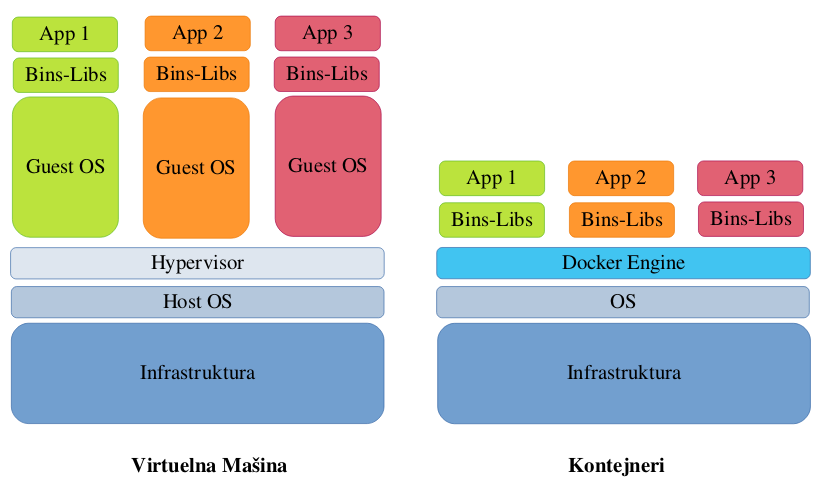
\includegraphics[width=\linewidth]{images/vm.png}
    \caption{Razlika između arhitekture Virtuelne Mašine a arhitekture kontejnera}
\end{figure}


\chapter{Literatura}
\sloppy
\printbibliography[heading=none]

\end{document}
